\begin{answer}
\begin{figure}[H]
    \centering
    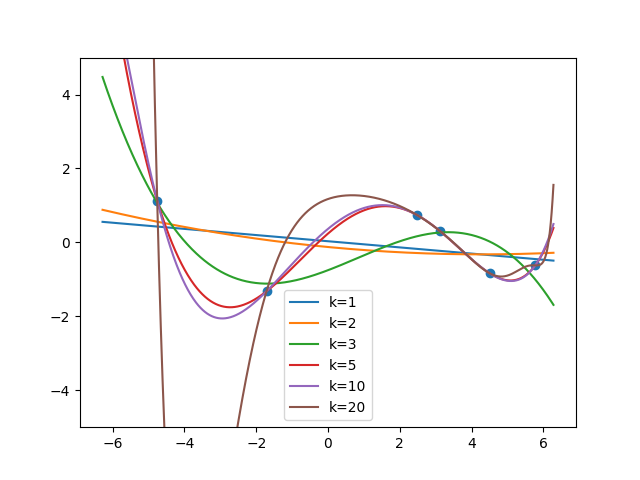
\includegraphics[width=9cm]{featuremaps/overfitting.png}
\end{figure}
For $n$ datapoints a polynomial of degree $n-1$ can perfectly interpolate the data. Therefore polynomials of degree $n-1$ can attain zero loss. There are 6 points in the data, and from the plot, we observe that the models with $k\ge 5$ fit the data perfectly.
\end{answer}
